\documentclass[9pt,twocolumn,twoside,lineno]{pnas-new}
% Use the lineno option to display guide line numbers if required.
% Note that the use of elements such as single-column equations
% may affect the guide line number alignment. 
\templatetype{pnasresearcharticle} % Choose template 
% {pnasresearcharticle} = Template for a two-column research article
% {pnasmathematics} = Template for a one-column mathematics article
% {pnasinvited} = Template for a PNAS invited submission

%\documentclass[12pt]{article}
%\usepackage[square,sort,comma,numbers]{natbib}
%\usepackage{times}
\usepackage[T1]{fontenc}
\usepackage[utf8]{inputenc}
%\usepackage[pdftex]{graphicx}
%\usepackage{caption}
%\captionsetup[figure]{justification=raggedright,labelfont=bf}
%\usepackage{fullpage} % 1" margins
\usepackage{tabu}
\usepackage{pdflscape}
%\usepackage{setspace}
%\setstretch{1.5}
%\usepackage{lineno}
%\usepackage{sectsty}
%\sectionfont{\nohang\centering\normalsize\sc}   % capitalize initial letters
%\subsectionfont{\nohang\centering\normalsize\rm\em}

% eat the colon so figures are labeled but have blank captions
% \makeatletter
% \renewcommand\fnum@figure[1]{\figurename~\thefigure\ignorespaces}
% \makeatother

%% Article

\title{Uplift-driven diversification in the Hengduan Mountains, a
  temperate biodiversity hotspot}

\author[a,b,1]{Yaowu Xing}
\author[a,c,1]{Richard H.\ Ree} 
% Use letters for affiliations, numbers to show equal authorship (if applicable) and to indicate the corresponding author
\affil[a]{Integrative Research Center, The Field Museum, 1400 South
  Lake Shore Drive, Chicago, Illinois 60605, USA}
\affil[b]{Xishuangbanna Tropical Botanical Garden, Chinese Academy of
  Sciences, Menglun Township, Mengla County, Yunnan 666303, China}
\affil[c]{National Institute of Ecology, 1210 Geumgang-ro,
  Maseo-myeon, Seocheon-gun, Chungcheongnam-do, South Korea}

% Please give the surname of the lead author for the running footer
\leadauthor{Xing} 

\significancestatement{Why do so many species occur in mountains? A
  popular but little-tested hypothesis is that tectonic uplift creates
  environmental conditions (new habitats, dispersal barriers, etc.)
  that increase the rate at which resident species divide and evolve
  to form new ones. In China's Hengduan Mountains region, a
  biodiversity hotspot uplifted over the last 8 million years, this
  rate does in fact show a significant increase during that time,
  relative to the rate for adjacent older mountains, and to the rate
  of species immigration. The Hengduan Mountains flora is thus made up
  disproportionately of species that evolved within the region during
  its uplift, supporting the original hypothesis and helping to
  explain the prevalence of mountains as global biodiversity
  hotspots.}

%\date{Yaowu Xing$^{1,2}$ and Richard H.\ Ree$^{1,3,*}$}

\authorcontributions{Y.X. and R.R. designed the research; Y.X. collected the
  data; Y.X. and R.R. analyzed the data; and Y.X. and R.R. wrote the paper.}

\authordeclaration{The authors declare no conflicts of interest.}

\equalauthors{\textsuperscript{1}Y.X. and R.R. contributed equally to this work.}

\correspondingauthor{\textsuperscript{2}To whom correspondence should be addressed. E-mail: \href{mailto:rree@fieldmuseum.org}{rree@fieldmuseum.org}}

\keywords{ biogeography $|$ vascular plants $|$ molecular clocks $|$ dispersal $|$ speciation }

\begin{abstract}
  A common hypothesis for the rich biodiversity found in mountains is
  uplift-driven diversification---that orogeny creates conditions
  favoring rapid \textit{in situ} speciation of resident lineages. We
  tested this hypothesis in the context of the Qinghai-Tibetan Plateau
  (QTP) and adjoining mountain ranges, using the phylogenetic and
  geographic histories of multiple groups of plants to infer the tempo
  (rate) and mode (colonization vs.\ \textit{in situ} diversification)
  of biotic assembly through time and across regions. We focused on
  the Hengduan Mountains region, which in comparison to the QTP and
  Himalayas was uplifted more recently (since the late Miocene), is
  smaller in area, and richer in species. The time-calibrated
  phylogenetic analyses showed that about 8 million years ago, the
  rate of \textit{in situ} diversification increased in the Hengduan
  Mountains, significantly exceeding that in the geologically older
  QTP and Himalayas. By contrast, in the QTP and Himalayas during the
  same period, the rate of \textit{in situ} diversification remained
  relatively flat, with colonization dominating lineage
  accumulation. The Hengduan Mountains flora was thus assembled
  disproportionately by recent \textit{in situ} diversification,
  temporally congruent with independent estimates of orogeny. This is
  the first study to show quantitative evidence for uplift-driven
  diversification in this region, and more generally, to test the
  hypothesis by comparing the rate and mode of biotic assembly jointly
  across time and space. It thus complements the more prevalent method
  of examining endemic radiations individually, and could be used as a
  template to augment such studies in other biodiversity hotspots.
\end{abstract}

\dates{This manuscript was compiled on \today}
\doi{\url{www.pnas.org/cgi/doi/10.1073/pnas.XXXXXXXXXX}}

\begin{document}
% \raggedright
% \parindent 0.5in

% Optional adjustment to line up main text (after abstract) of first page with line numbers, when using both lineno and twocolumn options.
% You should only change this length when you've finalised the article contents.
\verticaladjustment{-2pt}

\maketitle

\thispagestyle{firststyle}
\ifthenelse{\boolean{shortarticle}}{\ifthenelse{\boolean{singlecolumn}}{\abscontentformatted}{\abscontent}}{}

Central to understanding global patterns of biodiversity are
considerations of biotic assembly: for a given region, when and how
did resident species accumulate? Of primary interest is tempo (the
rate of accumulation) and mode (the process, whether by colonization
via dispersal, or \textit{in situ} lineage diversification). We wish
to know how and why these vary in time and space.

For mountains, well-known for harboring a disproportionate fraction of
terrestrial species, a common hypothesis is that of uplift-driven
diversification---that orogeny creates conditions favoring \textit{in
  situ} speciation of resident lineages
\citep{Hoorn2013,hughes2016,Wen2014,Favre2015,Lagomarsino2016,schwery2015}. Among
global biodiversity hotspots, the mountain ranges surrounding the
Qinghai-Tibetan Plateau (QTP) are unusual and enigmatic: they harbor
one of the world's richest temperate floras, and (unlike other
hotspots) they are neither tropical nor Mediterranean in
climate. Moreover, despite increasing interest from biogeographers,
their biotic assembly remains poorly understood
\citep{Favre2015,Wen2014,Hughes2015}. The mountains form 3 distinct
hotspots of biodiversity which respectively lie to the west, south,
and east of the QTP's central high desert: the Central Asian mountains
(Altai and Tianshan ranges), the Himalayas, and the Hengduan Mountains
region \citep{Favre2015}. Of these, the richest in plant diversity is
the Hengduan Mountains, with a vascular flora of about 12,000 species
in an area of about 500,000 km$^2$
\citep{Boufford2014,LiEtLi1993,Wu1988}. In this study, we seek to
better understand the origins of this remarkable flora through the
lens of historical biogeography. In particular, was \textit{in situ}
diversification accelerated by uplift of the Hengduan Mountains?


The geological history of the QTP and its surrounding ranges is
complex, and many details remain controversial, with different lines
of evidence often yielding conflicting inferences. However, some
points of consensus have emerged from recent syntheses
\citep{WangC2014,Favre2015,Deng2015,Renner2016}. One is that the
central plateau was uplifted first, forming a "proto-QTP" as early as
40 Mya, with subsequent outward extensions by the early Miocene
\citep{Rowley2006,WangC2014}. By the late Miocene, 8--10 Mya, all the
mountains surrounding the QTP to the south, west, and north had
reached their current elevations
\citep{Spicer2003,Fang2005,WangY2012,Deng2015}. By contrast, uplift of
the Hengduan Mountains region, at the southeastern margin, is
generally believed to have been rapid and recent, occurring mainly
between the late Miocene and late Pliocene
\citep{kirby2002,clark2005,WangE2012,Wang2014,Meng2016,SunB2011}.

The Hengduan Mountains are thus younger than the rest of the QTP and
relatively small in area, but conspicuously rich in species. If
floristic assembly tracks orogeny, this suggests an elevated tempo
since the late Miocene, compared to adjacent regions; but what of
mode? Either colonization, \textit{in situ} diversification, or both
processes must have been accelerated. In biogeographic studies of
QTP-associated clades, the hypothesis of uplift-driven \textit{in
  situ} diversification has been clearly favored over colonization,
being commonly invoked to explain phylogenetic and phylogeographic
divergences
\citep[e.g.,][]{LiuJ2006,WangY2009,ZhangJ2014,GaoY2013}. However,
conspicuously lacking from these studies are quantitative analyses
that explicitly measure rates of diversification and colonization, and
compare them across regions and time
\citep{Wen2014,Favre2015}. Consequently, the idea that uplift-driven
diversification has contributed disproportionately to floristic
assembly in the Hengduan Mountains has yet to be rigorously tested.

In this study we used the evolutionary histories of multiple plant
groups to study the floristic assembly of the Hengduan Mountains
region, focusing on comparisons to adjacent regions, especially the
Himalayas and other geologically older parts of the QTP
(Fig.~\ref{fig:map}). We inferred regional rates of diversification
and colonization through time from fossil-calibrated molecular
chronograms and reconstructions of ancestral range and rates of
lineage diversification, using data from 19 clades of vascular plants
chosen for their potential to inform the biogeographic history of the
Hengduan Mountains. Our primary aim was to discover the differences in
tempo and mode of biotic assembly that help account for the remarkable
diversity of the Hengduan flora.


\section*{Results}

\subsection*{Contrasting histories of floristic assembly}

Reconstructed biogeographic histories of the selected clades reveal
distinct patterns of floristic assembly across regions when plotted as
the cumulative number of colonization and \textit{in situ} speciation
events through time (Fig.~\ref{fig:cumevents}). Given geological and
paleontological evidence that the Hengduan Mountains are younger than
the Himalayas-QTP, we expected to find that its flora was assembled
more recently. Instead, we found surprisingly deep phylogenetic
histories of Hengduan occupancy, with initial assembly of its flora
pre-dating that of the Himalayas-QTP. In more than 95\% of the
pseudoreplicated joint histories, the earliest colonization event
occurs by 64 Ma for the Hengduan Mountains and by 59 Ma for the
Himalayas-QTP; \textit{in situ} speciation begins later, starting by
34 Ma and 19 Ma, respectively. By contrast, in temperate/boreal East
Asia, which was commonly reconstructed as the root ancestral area for
clades, \textit{in situ} speciation initially occurs by 155 Ma and
colonization initially occurs by 60 Ma.

For all regions, species accumulation by each process is approximately
exponential (log-linear) following initiation until about the last 8
Ma. During this earlier "constant" phase, assembly in both the
Hengduan Mountains and Himalayas-QTP is dominated by colonization,
while in temperate/boreal East Asia the dominant process is \textit{in
  situ} speciation. Following this phase, the assembly dynamics of the
Hengduan Mountains and Himalayas diverge considerably, with relatively
little change in temperate/boreal East Asia. In the Hengduan
Mountains, the cumulative number of \textit{in situ} speciation events
overtakes that of colonization around 8 Ma, and by the present, the
median number is 508 versus 335. In the Himalayas-QTP, \textit{in
  situ} speciation never overtakes colonization, and by the present
the median number of events is 192 versus 411. The relative
contribution of \textit{in situ} speciation to floristic assembly is
thus $508/(508+335) = 0.603$ for the Hengduan Mountains, and
$192/(192+411) = 0.318$ for the Himalayas-QTP. In other words,
\textit{in situ} speciation has contributed almost twice as much to
the assembly of the Hengduan Mountains flora as it has to the
Himalayas-QTP flora, especially since the late Miocene.

\subsection*{Regional rates of \textit{in situ} speciation and
  dispersal through time}

The rate of \textit{in situ} speciation for the Hengduan Mountains
region, in events per resident lineage per Ma, increased almost
twofold over the past 10 Ma, while for the Himalayas-QTP, it remained
more or less constant (Fig.~\ref{fig:speciation}). Dispersal rates
between the Hengduan Mountains and Himalayas-QTP increase gradually
over the last 4--5 Ma, and sharply in the last 1 Ma. By contrast,
dispersal from each region to temperate/boreal East Asia increases
only slightly in the same time period (Fig.~\ref{fig:dispersal}).

\subsection*{Shifts in diversification rate}

Seven out of the 19 clades showed strong evidence (Bayes factor > 15)
for one or more shifts in diversification regime
(Table~\ref{table:bammbayesfactors}). However, inspection of
branch-specific evidence (the cumulative probability of occurring in
the credible set of shift configurations, and the marginal odds ratio
in favor of a shift) in light of ancestral-range reconstructions does
not reveal any clear geographic patterns in the phylogenetic locations
of regime shifts (Fig.~S2). That is, across clades, macroevolutionary
jumps in diversification rate are not obviously associated with the
colonization or occupancy of any particular region.

A notable exception to this general pattern is \emph{Rhododendron}, in
which results from BAMM and Lagrange suggest that in a window of about
9--15 Ma, net diversification increased independently in 2 clades that
each originated in the Hengduan region and are currently dominated by
Hengduan species (Fig.~\ref{fig:rhododendron}). In \emph{Saussurea},
an increase in net diversification is inferred about 1.7 Ma along the
stem of a branch containing most of the clade's Hengduan species
(Fig.~S2O). Similarly, in Delphineae, 2 separate increases are
inferred in clades that are ancestrally Hengduan and together hold
most of the Hengduan species; however the times of these rate shifts
(about 28 Ma and 37 Ma, respectively) pre-date the uplift of the
Hengduan Mountains (Fig.~S2D). Finally, in \emph{Isodon} and the
\emph{Ligularia-Cremanthodium-Parasenecio} complex, branch-specific
measures show one increase in net diversification for each clade in
the context of Hengduan ancestry about 7 and 5 Ma, respectively, but
in both cases, models with regime shifts are not supported by Bayes
factors, and the Hengduan Mountains region is reconstructed as
ancestral across most of the phylogeny, rendering the geographic
context of the shift less informative.

\section*{Discussion}

Our analysis is the first to quantify the relative contributions of
\textit{in situ} lineage diversification and colonization to the
assembly of one of the world's richest temperate floras, that of the
Hengduan Mountains. We expected regional differences to reflect
contrasting times of orogeny; in particular, the prediction of the
uplift-driven diversification hypothesis that \textit{in situ}
speciation increases with mountain-building activity. In this context,
the late Miocene emerges as an important reference point, as previous
studies of geology and paleontology indicate that the Hengduan
Mountains achieved their current height only after this time, while
the Himalayas and central QTP did so before
\citep{WangY2012,Wang2014,Spicer2003,Favre2015,Renner2016}. Here, our
phylogenetic inferences, which make no prior assumptions about the
timing of geological events, show that after about 8 Ma, the rate of
\textit{in situ} diversification increased in the Hengduan Mountains,
yielding a remarkable inflection point at which cumulative speciation
overtakes colonization. This indicates that the Hengduan Mountains
flora has been assembled disproportionately by recent \textit{in situ}
diversification that coincides temporally with independent estimates
of orogeny.

We do not find a similar signature of accelerated \textit{in situ}
diversification for the Himalayas-QTP region, as might be expected
from rapid Himalayan orogeny during the early to middle Miocene
\citep{searle2011,Spicer2003,Wang2014}. It is possible that no such
pulse of diversification occurred, e.g., if uplift of the Himalayas
was more gradual. Alternatively, we could simply lack the statistical
power to detect it, due to the masking effects of treating the older
QTP and the younger Himalayas as a single region, the greater
uncertainty associated with estimating clade ages and ancestral ranges
in deeper time, and/or extinction and turnover in the Himalayas-QTP
flora.

In a recent review, Renner \citep{Renner2016} argued that numerous
phylogenetic studies have misinterpreted the Earth sciences literature
and incorrectly attributed relatively young (Miocene and later)
estimates of lineage divergence to QTP uplift, and recommended that
``Biogeographical discussions should also keep in mind expected
differences in the biota of the TP and those in the Himalayas, the
Kunlun range to the N, the Pamir and Karakoram to the W, and Hengduan
Mountains to the E'' \citep[][p.~7]{Renner2016}. Here, our focus on
distinguishing the younger and more species-rich Hengduan Mountains
region from the Himalayas-QTP is in the spirit of that advice, and our
results suggest that at least some of the referenced cases of
diversification could be more accurately interpreted as coincident
with orogeny of the Hengduan region, not the older QTP. Indeed,
several of the studies cited in Renner \citep{Renner2016} are the
original sources of molecular data for the clades analyzed here, and
include many Hengduan species. It thus seems important to emphasize
that, despite precedent in the literature for considering the Hengduan
Mountains to be simply part of a greater biogeographic region that
includes the Himalayas and QTP
\citep[e.g.][]{ZhangJ2014,Nie2013,GaoY2013,Matuszak2016}, the Hengduan
region actually has a very distinct history of assembly that reflects
its younger age.

% From Fig.2, speciation rate of Himalayas also increased until around 8 Ma, and keep constant since then. This probably due to Himalayas already reached its current elevation.

%Surpringly, our results indicate Himalayas-QTP flora was assembled later (Fig **). Ideally, bring paleontological evidence to bear on assembly/diversification questions - but the record is sparse. The exact time of onset of current biome remains unclear.

% MAIN POINT: temporal shifts (increases) in diversification in the absence of statistically significant endemic radiations

%\textbf{Drivers of Hengduan diversification.}---
Why did \textit{in situ} diversification in the Hengduan Mountains
increase since the late Miocene, and more specifically, to what extent
was it driven by orogeny? Further studies are needed. One might look
for contrasts between the Hengduan Mountains and adjacent regions in
the evolution of ecological traits and environmental tolerances
\citep[e.g.,][]{liu2016} across multiple clades. These may reveal, for
example, the extent to which speciation within a region is associated
with adaptive divergence and niche-filling, as opposed to nonadaptive
processes such as genetic isolation and drift arising from dispersal
limitation and topographic effects (vicariance, emergence of sky
islands, etc.). These analyses would require denser and more
fine-grained taxonomic and geographic sampling than was possible here,
in addition to the requisite trait data. However, we suspect that
evidence for common processes will prove elusive, as the proximate
causes of diversification are likely to be idiosyncratic, and involve
a variety of contingencies and associated variables
\citep[e.g.,][]{donoghue2015,bouchenak2015}. For many clades, factors
unrelated to uplift \emph{per se}, such as biotic interactions, are
almost certain to have played important roles
\citep{Luebert2014,Wen2014,Renner2016}. For example, in
\emph{Pedicularis} (Orobanchaceae), diversification of the many
Hengduan species may have been facilitated by recurrent divergence in
floral traits associated with pollinator sharing and reproductive
interference \citep[e.g.,][]{eaton2012}, in combination with other
mechanisms promoting population isolation, including uplift and
associated aspects of landscape and resource heterogeneity.

% Aridification and global cooling as a result of orogeny (see reviews in \citealt{MiaoY2012}) may be an important factor influencing the diversification of plants on the QTP.

A coarser-grained view is that diversification in the Hengduan region
reflects a macroevolutionary response to the rapid expansion of moist
temperate montane and alpine habitats in the late Miocene. At this
level the effects of orogeny and climate change are not clearly
separable, as they concurrently and jointly set a stage of
ecological/evolutionary opportunity. During the early to middle
Miocene, the southern QTP had already achieved its current elevation
\citep{Spicer2003} and was covered by coniferous and deciduous-leaved
forests
\citep{SunJ2014,LiH1976}% , and limited paleobotanical evidence suggests that the entire Himalayas-QTP region may have experienced a dramatic shift in vegetation after the middle Miocene
. As Hengduan uplift proceeded, falling temperatures would have driven
the treeline lower, increasing the extent of shrublands, meadows, and
scree slopes---habitats where most of the species in our data set
occur and would have diversified. Similar changes would also have
occurred in the Himalayas and QTP, but in comparison to those areas,
moisture in the Hengduan region would have been abundant, as by then,
the summer monsoon was established, and the central QTP and Central
Asian interior had aridified \citep[see][]{Renner2016}. This predicts
that carrying capacities---and by extension, diversification
potential---of the Hengduan region's newly formed habitats were
enhanced by greater summer rainfall.

% Accounting for the effect of Pleistocene climate fluctuations

While not a driver of diversification \textit{per se}, it is important
to consider the effects of glaciation and climatic oscillations during
the Pleistocene, and the possibility that our results can be
explained, at least in part, by regional differences in extinction
caused by these factors. In the Hengduan region, the north-south
orientation of major valleys suggests that extinction was relatively
low, as species would have been able to persist by migrating
relatively unhindered toward southern ice-free areas during glacial
cycles; as a result, the region's history of \textit{in situ}
diversification would be better preserved in time-calibrated
phylogenies, simply because fewer branches would have been ``pruned''
by extinction. By contrast, in the Himalayas-QTP, the east-west
orientation of valleys would have inhibited southern displacement,
leading to greater extinction. In this case, the pruning effect of
extinction would yield lower estimates of \textit{in situ}
diversification during the Pleistocene.

This pattern is probably not due solely to differences in glacial
extent. Numerous studies of species distributions
\citep[e.g.,][]{srinivasan2014,lopez2011} and phylogeography
\citep[e.g.,][]{CunY2010,WangBS2011,lei2014,meng2015} support the idea
that refugia occurred along the southeastern margin of the QTP as well
as in areas further west and north, even at high elevation
\citep[e.g.,][]{wang2009,sun2010,opgenoorth2010}. This aligns with
geological evidence that ice-free areas were present across the QTP
and adjacent mountains throughout the Quaternary
\citep[see][]{owen2014}. It may be that greater Pleistocene extinction
in the Himalayas-QTP compared to the Hengduan region was driven as
much (or more) by aridification as glaciation, as the former
experienced reduced summer monsoon strength during interglacials
\citep{owen2008}.

These effects may be reflected in temporal patterns of dispersal
between the Hengduan Mountains and Himalayas-QTP. The older age of the
latter predicts that its flora should have been an early source of
lineage dispersal to the younger Hengduan Mountains. However, we do
not find any marked asymmetry in dispersal between these regions
through the end of the Miocene; instead, rates in both directions are
relatively low and increase only gradually until about 2--3 Ma, when
both increase more sharply, but more so from the Hengduan Mountains to
the Himalayas-QTP (Fig.~\ref{fig:dispersal}). That is, in the
Quaternary, the Hengduan Mountains appear to have acted as a
biogeographic source, from which lineages buffered from extinction
colonized the relatively depauperate regions to the west and
north. % This may reflect phylogeographic evidence that the Hengduan Mountains flora was likely buffered from extinction during Quaternary glacial cycles, with subsequent westward range expansion/recolonization of the Himalayas and QTP \citep[e.g.,][]{WangBS2011,CunY2010}.

% even paleoelevational recontruction suggesting this regions already reached their current elevation by then . The onset and diversification of alpine biome may be much later than the uplift.

% More generally, it seems reasonable to view uplift and climate change as primary drivers of expanding ecological opportunities for temperate-montane species in the Hengduan region in the late Miocene.

%\textbf{Comparisons to other taxa, mountains, and hotspots.}

Other than plants, the group that has received the most biogeographic
scrutiny in relation to the QTP and adjacent regions is birds, which
present similar patterns \citep[see][]{packert2015}, notably that in
the species-rich Hengduan Mountains region and adjacent forests of SE
Asia, \textit{in situ} diversification during and subsequent to the
Miocene led to repeated colonization of the Himalayas and QTP
\citep[e.g.,][]{liu2016,tietze2013,johansson2007}. In the Himalayas,
the lack of \textit{in situ} diversification of songbirds has been
attributed to the filling of niches by pre-adapted colonizing lineages
\citep{price2014}.

% In this study we attempt to place the Hengduan Mountains flora in
% historical biogeographic context through the joint analysis of
% representative clades. The picture that emerges is one in which
% \textit{in situ} diversification accelerates relative to
% colonization around the time orogeny is believed to have started.

% To what extent do our results reflect general features of how
% biodiversity hotspots, especially those associated with mountains,
% are assembled?

% In this study we analyze the assembly of a biodiversity hotspot
% using a comparative framework of 4 dimensions: tempo (rates of
% biogeographic events), mode (\textit{in situ} diversification versus
% colonization), time

Among studies inferring biodiversity hotspot assembly from multiple
clades, quantitative analyses of \textit{in situ} diversification
and/or colonization are still rare, and ours is the first to estimate
rates of both processes through time and across regions. This
comparative framework has allowed us to characterize, at a very basic
level, changes in the tempo (rate) and mode (process) of biotic
assembly in relation to independently-inferred timelines of regional
orogeny and climate change. By contrast, studies of other hotspots
have tended to focus on single regions or biomes, and subsets of these
dimensions (time, space, tempo, and mode). For example, the high
species diversity in the California Floristic Province is associated
with lower rates of extinction more than elevated speciation or
immigration, using models in which rates of lineage birth, death, and
movement are dependent on geographic occupancy but not time
\citep{lancaster2013}. Assembly of the Cerrado biome in Brazil has
been characterized by recent (late Miocene onwards) \textit{in situ}
adaptation of lineages to fire resistance \citep{simon2009}, with some
clades, especially in the campos rupestres highlands, showing evidence
of endemic radiation (e.g., \textit{Mimosa}
\citep{koenen2013,simon2009}, \textit{Calliandra} \citep{souza2013},
and \textit{Chamaecrista} \citep{rando2015}). In the Páramo biome of
the Andes, analyses of net diversification (but not immigration)
yielded the highest average rate compared to eight other hotspots, and
appears driven more by Pleistocene climate oscillations than orogeny
\citep{Madrinan2013}. Clearly, for the Hengduan Mountains, much
remains to be studied about how patterns of assembly through time
break down at a finer scale of particular biomes and habitats within
the region.

The Andes, perhaps the world's richest mountain hotspot
\citep{hughes2016}, are a compelling subject for comparison to the
present results. The tropical montane/alpine habitats of the Andes are
geographically isolated, whereas the temperate Hengduan region is
embedded in a network of high mountains surrounding the QTP, and
proximate to cool high-latitude habitats. It thus stands to reason
that dispersal figures prominently in Hengduan biotic assembly,
compared to the Andes, in which endemic radiations are the more
dominant pattern
\citep[e.g.,][]{pennington2010,Lagomarsino2016,Hughes2015,Luebert2014,Hughes2006}.

Prevalence of dispersal is likely the underlying reason that we find
little evidence of macroevolutionary jumps in diversification rate
associated with Hengduan colonization in individual clades. In our
phylogenies, clades tend not to be entirely endemic to the Hengduan
Mountains or Himalayas-QTP; dispersal is common, and reflects the fact
that these regions are not defined by differences in biome, but share
broad physiographic similarities that presumably have facilitated
biogeographic exchange. That is, dispersal between these regions
should not necessarily require extensive ecophysiological adaptations
that may be difficult to evolve \citep{Donoghue2014}, countering
expectations of infrequent colonization events followed by endemic
radiations \citep[cf.][]{Hughes2006}. For this reason our data are
perhaps not well-suited for BAMM, which models diversification shifts
as relatively rare events. Moreover, the link between dispersal events
and shifts in diversification regime is further obscured by the
inherent uncertainty associated with inferring their phylogenetic
locations. The most appropriate interpretation may simply be that the
signal of higher diversification in the Hengduan region is more or
less diffuse across clades, and emerges only when their biogeographic
histories are considered jointly. This helps explain why previous
analyses of single clades have not yielded the pattern inferred here.

The validity of our results hinges on the degree to which the data are
representative of the focal regions (Hengduan Mountains and
Himalayas-QTP). The clades we selected span a wide taxonomic range,
and the species exhibit a diversity of growth forms, life histories,
and habitat preferences. Taxon sampling, while incomplete, is not
generally biased with respect to the focal regions (Table S1), and
therefore should not unduly affect inferences of the relative rates of
assembly processes across regions. We also expect the phylogenetic
distribution of unsampled species within each clade to be effectively
random, which means that reconstructed phylogenies would tend to be
missing more nodes---and thus inferred biogeographic events---closer
to the present. In other words, the extent to which we have
underestimated the frequencies of those events is likely greater in
the Pliocene and Quaternary than in the Miocene and earlier.

Another potential source of error is in the demarcation of discrete
areas as required for biogeographic analysis. While the QTP,
Himalayas, and Hengduan Mountains may have broadly distinct orogenic
histories, this does not translate into clearly defined borders; and
to the extent such borders existed, they surely would have shifted
through time, leading to ambiguity in the present. Our definitions of
these areas are thus necessarily somewhat subjective, and represent
our best attempts to capture the essential elements of this complex
system. That being said, our results are robust to the treatment of
the Himalayas and QTP as a single biogeographic area; an analyis of
recoded species range data treating them as separate areas yielded the
same signature of uplift-driven Hengduan diversification (see
\textit{SI Text} and Figures S3--S5).

%\section{Materials and Methods}

\subsection{Clade selection and phylogeny reconstruction}

Our criteria were that each clade (1) included a substantial number of species that occur in the Hengduan Mountains, as well as their closest known relatives in other biogeographic regions; (2) had sufficient molecular data available to infer a phylogeny that was broadly representative of the clade's taxonomic diversity and geographic range; and (3) had fossil data suitable for molecular clock calibration or secondary calibrations inferred from fossil dated phylogenies. We found 18 clades---16 of angiosperms and one each of gymnosperms (Pinaceae) and ferns (Microsorioideae)---that met these criteria. The combined taxon sample included a total of 3,262 ingroup species, of which 899 occur in the Hengduan Mountains region, 624 in the Himalayas-QTP, and 1,165 in the remainder of temperate/boreal East Asia (see \textit{Delimitation of biogeographic regions}). Of these, about 370 species are shared by the Hengduan Mountains and Himalayas-QTP regions. Across clades, the proportion of species sampled ranged from 20--97\% globally and 40--97\% for the Hengduan Mountains region (Table S1).

For each clade, we assembled molecular sequence alignments (Table S2; \textit{Appendix 1}) and fossil calibration data, and used relaxed molecular clock models implemented in BEAST 1.8 \citep{Drummond2012} or 2.0 \citep{Bouckaert2014} to generate a Bayesian posterior sample of time-calibrated phylogenies and the associated maximum-clade-credibility tree.  Detailed information is provided in \textit{SI Materials and Methods}.

%, representing approximately XX\%, YY\%, and ZZ\% of the vascular flora of each region (SI REF).

\subsection{Inference of range evolution and lineage diversification}

\subsubsection{Delimitation of biogeographic regions}

We defined 11 biogeographic regions (Fig.~S1), balancing considerations of model complexity, the need to accommodate the global distributions of the selected clades, and the granularity of our species range data. Of primary importance was distinguishing the Hengduan Mountains region from the geologically older parts of the QTP, especially the Himalayas. To that end, our definition of the Hengduan Mountains region follows \citet{Boufford2014}, and is bounded to the west by the Yarlung Tsangpo River in eastern Xizang (Tibet), to the northwest by the high plateau in Qinghai, to the north by the Tao River in southern Gansu, to the east by the Sichuan Basin, and to the south by subtropical forests and the Yunnan–Guizhou Plateau. As a primary point of comparison, we defined the ``Himalayas-QTP'' region as including the plateau itself, the Himalayas to the south, the Kunlun Mountains to the north, and the Qilian Mountains to the northeast. The other regions we defined are: temperate/boreal East Asia (the eastern boreal part of Russia and temperate regions of East Asia, including Japan and Taiwan); central/western Asia (including the Xinjiang Uyghur Autonomous Region to the south of Kunlun Range); southeast Asia (including tropical regions of China, Malesia, and Papuasia); Australasia (Australia, New Zealand, and the southwestern Pacific); India (south of the Himalyas, including Sri Lanka); Africa; Europe; North America; and South America (south of the Panama Canal). We scored the geographic range of each sampled species as its presence or absence in these regions based on floras, online databases, and published data sets (\textit{Dataset S1}; see also \textit{SI Materials and Methods}).

\subsubsection{Ancestral range reconstruction}

We set up a DEC model of range evolution in Lagrange \citep{Ree2005,Ree2008}, specifying a region-adjacency matrix that defined the valid set of spatially contiguous ranges. We explicitly avoided placing any temporal constraints on dispersal, so that biogeographic inferences were independent of prior beliefs about the ages of the Hengduan Mountains or Himalayas-QTP regions. For each clade, we used the model to infer a distribution of phylogenetic histories of biogeographic events. A single history for a clade was generated by sampling a chronogram from its Bayesian posterior distribution, estimating the maximum-likelihood set of ancestral ranges (geographic speciation scenarios) at internal nodes, and randomly interpolating parsimonious sequences of dispersal and local extinction events along branches having different ancestral and descendant ranges. This yielded a complete chronology of biogeographic events, i.e., where and when ancestral lineages moved and underwent speciation and local extinction. To account for phylogenetic uncertainty, one history was generated for each of 500 chronograms drawn randomly from the posterior for each clade. For further details, see \textit{SI Materials and Methods}.

\subsubsection{Regional assembly processes through time}

We focused our analysis on the dynamics of the Hengduan Mountains region in comparison to the Himalayas-QTP and temperate East Asia. Our objective was to estimate, for each region, rates of \textit{in situ} diversification and colonization and their cumulative contributions to biotic assembly through time. Taking the biogeographic histories of clades from the ancestral-range analysis, we generated 500 pseudoreplicated joint histories---sets of one history drawn randomly from each clade's pool without replacement. From each joint history, we extracted the chronology of \textit{in situ} speciation, colonization, and local extinction events affecting the 3 regions of interest and binned them into 1 Myr periods. This allowed region-specific estimates of assembly processes through time. We calculated rolling estimates of \textit{in situ} speciation rates as $\lambda(t) = s(t)/n(t-1)$, where $s(t)$ is the number of \textit{in situ} speciation events inferred in a region in a 1-Myr period $t$ and $n(t-1)$ is the number of inferred lineages in the region in the previous period (the cumulative sum of \textit{in situ} speciation and colonization minus local extinction). We also calculated rolling rates of colonization between regions as $d_{ij}(t) = c_{ij}(t)/n_i(t-1)$, where $c_{ij}(t)$ is the number of inferred colonization events of area $j$ from area $i$. For all estimates, confidence intervals (5--95\% quantiles) were calculated from the pseudoreplicated joint histories. Further details are provided in the \textit{SI Materials and Methods}.

\subsubsection{Geography-independent rates of diversification}

To complement the regional-process analysis and to better understand heterogeneity in rates of lineage diversification independently of geography, we generated Bayesian inferences of diversification rate for each clade using BAMM \cite{Rabosky2014}, which uses Markov chain Monte Carlo procedures to jointly estimate the number, parameters, and locations of distinct macroevolutionary regimes (rates of lineage birth and death, possibly time-dependent) on a phylogenetic tree. BAMM is able to account statistically for incomplete taxon sampling, so we assigned sampling fractions at the finest level of taxonomic resolution possible: this was generally at the level of genus, but at the level of section for \textit{Rhododendron} and \textit{Acer}. In cases where genera were not confidently resolved as monophyletic, we assigned sampling fractions at the higher taxonomic levels (tribe and subfamily). We ran each BAMM MCMC for 100 million generations with a sampling frequency of 1000 and assessed convergence by visually inspecting plots of the likelihood trace and calculating the effective sample size after discarding the first 10\% of the run as burn-in. We identified the 95\% credible set of distinct shift configurations and the overall best set of rate shifts given the data using the BAMMtools package in R \cite{Rabosky2014}.


\clearpage

\begin{landscape}

\begin{table}[th]
  \caption{Bayes factor support for shifts in diversification in sampled clades, relative to the null hypothesis of no shifts. Strong support (value $>$ 15) is indicated in bold.}
  \begin{tabu} to \linewidth {X[-2,l,b]X[-1,r,b]X[-1,r,b]X[-1,r,b]X[-1,r,b]X[-1,r,b]X[-1,r,b]X[-1,r,b]X[-1,r,b]X[-1,r,b]X[-1,r,b]X[-1,r,b]}
    \hline
    & \multicolumn{11}{c}{number of regime shifts} \\
    Clade                               & 1               & 2                & 3                & 4                & 5                & 6                & 7                & 8                & 9                & 10              & 11     \\
    \hline
    \textbf{\textit{Acer}}              & \textbf{31.76}  & \textbf{71.62}   & \textbf{26.07}   & 5.59             & 1.05             & 0.12             &                  &                  &                  &                 &        \\
    \textbf{\textit{Allium}}            & 14.24           & \textbf{182.48}  & \textbf{1048.16} & \textbf{3836.48} & \textbf{6668.16} & \textbf{7038.72} & \textbf{5401.60} & \textbf{3015.68} & \textbf{1382.40} & \textbf{409.60} & 163.84 \\
    Clematidinae+Anemoninae             & 6.74            & 6.82             & 4.10             & 1.72             & 0.44             & 0.16             & 0.05             &                  &                  &                 &        \\
    \textit{Cyananthus}                 & 0.96            & 0.52             & 0.18             & 0.06             & 0.02             & 0.00             &                  &                  &                  &                 &        \\
    \textbf{Delphineae}                 & \textbf{377.43} & \textbf{5871.71} & \textbf{6889.71} & \textbf{4316.57} & \textbf{1872.00} & \textbf{566.86}  & \textbf{137.14}  & \textbf{36.57}   &                  &                 &        \\
    \textit{Isodon}                     & 8.18            & 8.60             & 5.23             & 2.23             & 0.94             & 0.19             & 0.06             &                  &                  &                 &        \\
    \textit{Ligularia-Cremanthodium-Parasenecio} complex                  & 1.64            & 1.41             & 0.80             & 0.32             & 0.12             & 0.04             & 0.01             &                  &                  &                 &        \\
    \textit{Lilium}+\textit{Nomocharis} & 0.17            & 0.041            & 0.01             &                  &                  &                  &                  &                  &                  &                 &        \\
    \textit{Meconopsis}                 & 0.77            & 0.32             & 0.10             & 0.02             & 0.01             &                  &                  &                  &                  &                 &        \\
    Microsoroideae                      & 3.83            & 4.37             & 2.79             & 1.19             & 0.38             & 0.11             & 0.07             &                  &                  &                 &        \\
    \textbf{Pinaceae}                   & \textbf{40.78}  & \textbf{29.36}   & 10.15            & 2.17             & 0.34             & 0.05             &                  &                  &                  &                 &        \\
    \textbf{Polygoneae}                 & \textbf{550.12} & \textbf{1841.18} & \textbf{7241.41} & \textbf{8086.59} & \textbf{5225.41} & \textbf{2304.00} & \textbf{783.06}  & \textbf{165.65}  &                  &                 &        \\
    Primulaceae                         & 2.13            & 2.18             & 1.54             & 0.77             & 0.36             & 0.09             & 0.06             & 0.02             &                  &                 &        \\
    \textit{Rhodiola}                   & 1.94            & 1.92             & 1.33             & 0.71             & 0.26             & 0.08             & 0.02             &                  &                  &                 &        \\
    \textbf{\textit{Rhododendron}}      & \textbf{17.76}  & \textbf{87.97}   & \textbf{247.00}  & \textbf{289.51}  & \textbf{215.75}  & \textbf{111.64}  & \textbf{40.47}   & 9.76             & 2.30             &                 &        \\
    \textit{Rosa}                       & 1.31            & 0.90             & 0.42             & 0.18             & 0.03             & 0.01             &                  &                  &                  &                 &        \\
    \textbf{\textit{Saussurea}}         & 7.30            & \textbf{20.21}   & \textbf{21.68}   & 13.56            & 6.26             & 2.01             & 0.35             &                  &                  &                 &        \\
    Saxifragaceae+Grossulariaceae       & 1.91            & 1.52             & 0.72             & 0.26             & 0.04             & 0.00             &                  &                  &                  &                 &        \\
    \textit{Thalictrum}                 & 1.57            & 1.25             & 0.67             & 0.28             & 0.10             & 0.02             & 0.01             &                  &                  &                 &        \\
    \hline
    
  \end{tabu}
  \label{table:bammbayesfactors}
\end{table}

\end{landscape}

%%% Local Variables: 
%%% mode: latex
%%% TeX-master: "master"
%%% End: 


\begin{figure}
\centering
\includegraphics[width=.99\linewidth]{qtp-map.pdf}
\caption{Map of the Hengduan Mountains region in relation to the
  Qinghai-Tibetan Plateau and Himalayas.}
\label{fig:map}
\end{figure}

\begin{figure}
\centering
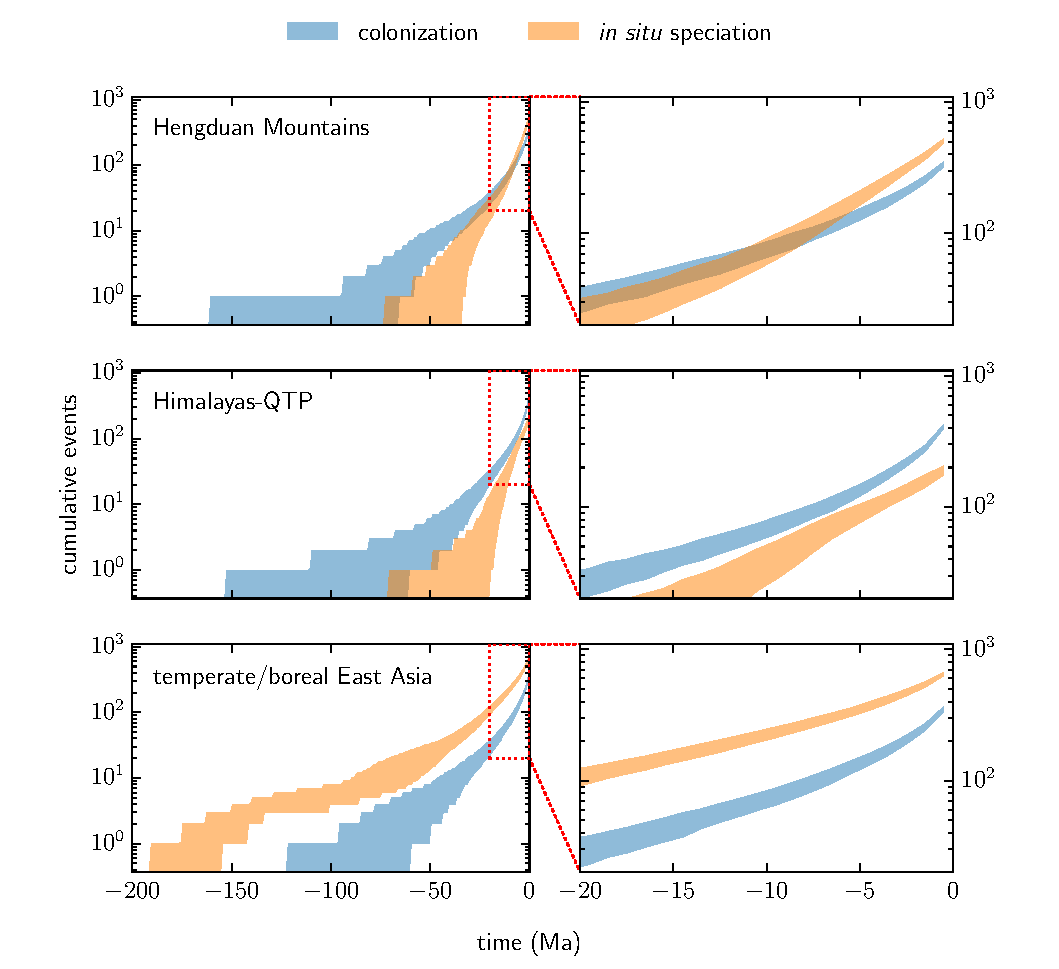
\includegraphics[width=.99\linewidth]{cumulative_events.pdf}
\caption{Assembly of regional floras by colonization and \textit{in
    situ} speciation events in 19 plant clades, inferred from
  ancestral-range reconstructions on time-calibrated molecular
  phylogenies. Shaded regions indicate the 5--95\% quantile intervals
  for the cumulative number of events through time from 500
  pseudoreplicated joint biogeographic histories designed to account
  for phylogenetic uncertainty (see text). Panels on the right focus
  on the last 20 Ma, in which differences in regional assembly are
  most apparent. In the Hengduan Mountains region, cumulative
  \textit{in situ} speciation overtakes colonization about 8 Ma,
  whereas for the Himalayas-QTP, colonization remains the dominant
  process. \textit{In situ} speciation thus appears to have played a
  disproportionately large role in assembling the Hengduan Mountains
  flora since the late Miocene compared to the Himalayas-QTP,
  consistent with the theory of uplift-driven diversification in the
  Hengduan Mountains region.}
\label{fig:cumevents}
\end{figure}

\begin{figure}
\centering
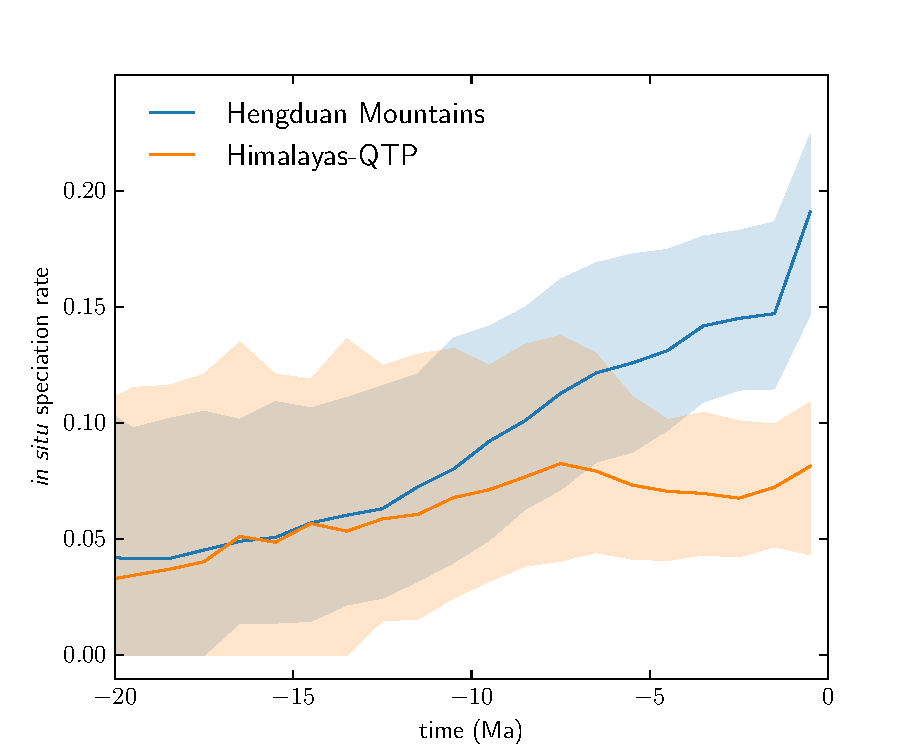
\includegraphics[width=.99\linewidth]{speciation_rates.pdf}
\caption{Rolling estimates of \textit{in situ} speciation rates
  through time for the Hengduan Mountains and Himalayas-QTP regions
  from inferred biogeographic histories of 19 plant clades. Lines
  indicate medians and shaded areas indicate 5--95\% quantile
  intervals from 500 pseudoreplicated joint histories designed to
  account for phylogenetic uncertainty (see text). Regional rates
  begin to diverge about 8 Ma, with the Hengduan Mountains showing a
  striking increase in \textit{in situ} speciation relative to the
  Himalayas-QTP.}
\label{fig:speciation}
\end{figure}

\begin{figure}
\centering
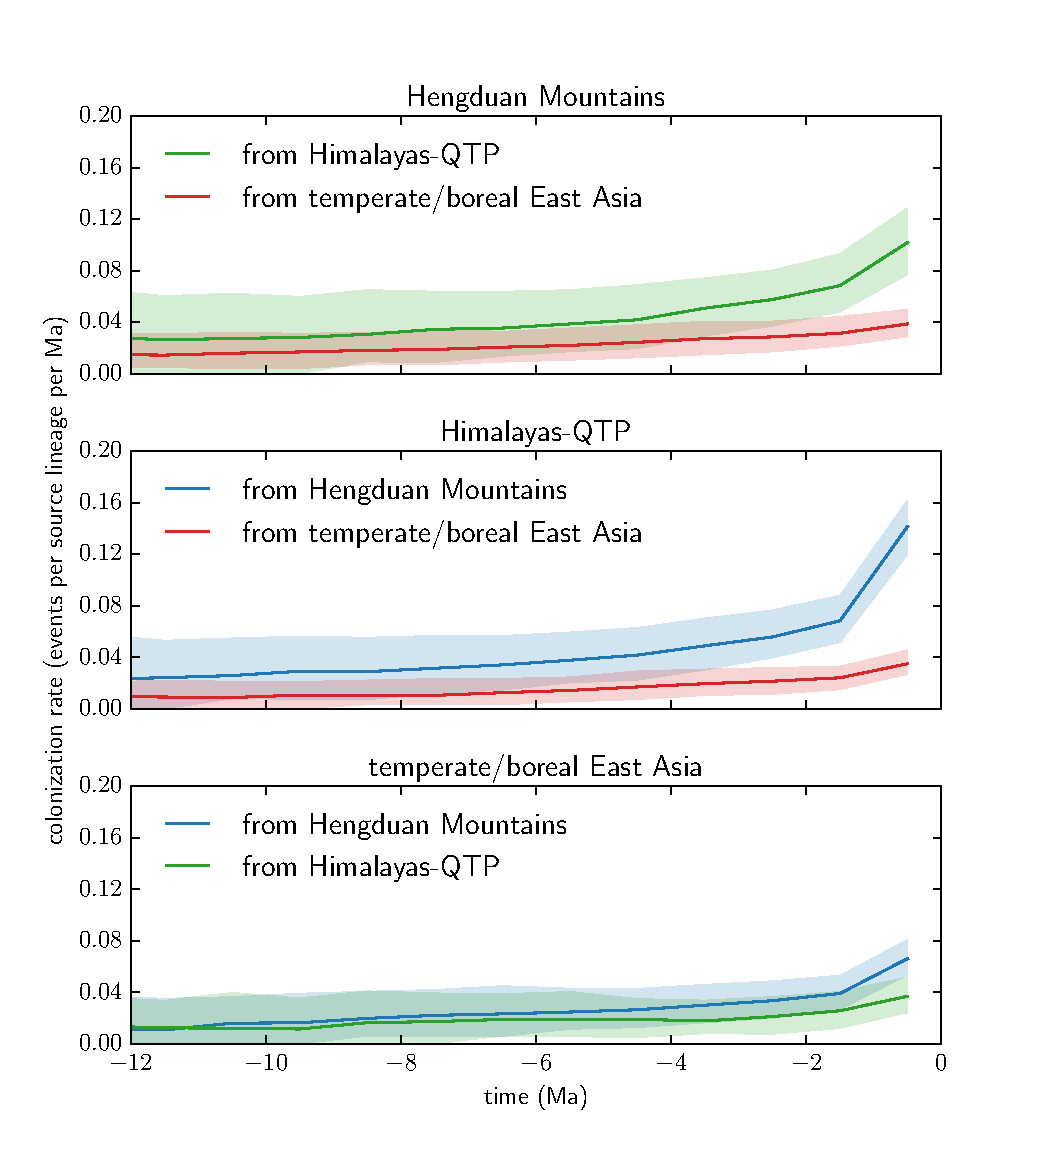
\includegraphics[width=.99\linewidth]{dispersal_rates.pdf}
\caption{Rolling estimates of colonization rates through time for the
  Hengduan Mountains, Himalayas-QTP, and temperate/boreal East Asia
  regions from inferred biogeographic histories of 19 plant
  clades. Lines indicate medians and shaded areas indicate 5–95\%
  quantile intervals from 500 pseudoreplicated joint histories
  designed to account for phylogenetic uncertainty (see
  text). Dispersal between the Hengduan Mountains and Himalayas-QTP
  increases in the last 2 Ma relative to dispersal between either
  region and temperate/boreal East Asia.}
\label{fig:dispersal}
\end{figure}

\begin{figure}
\centering
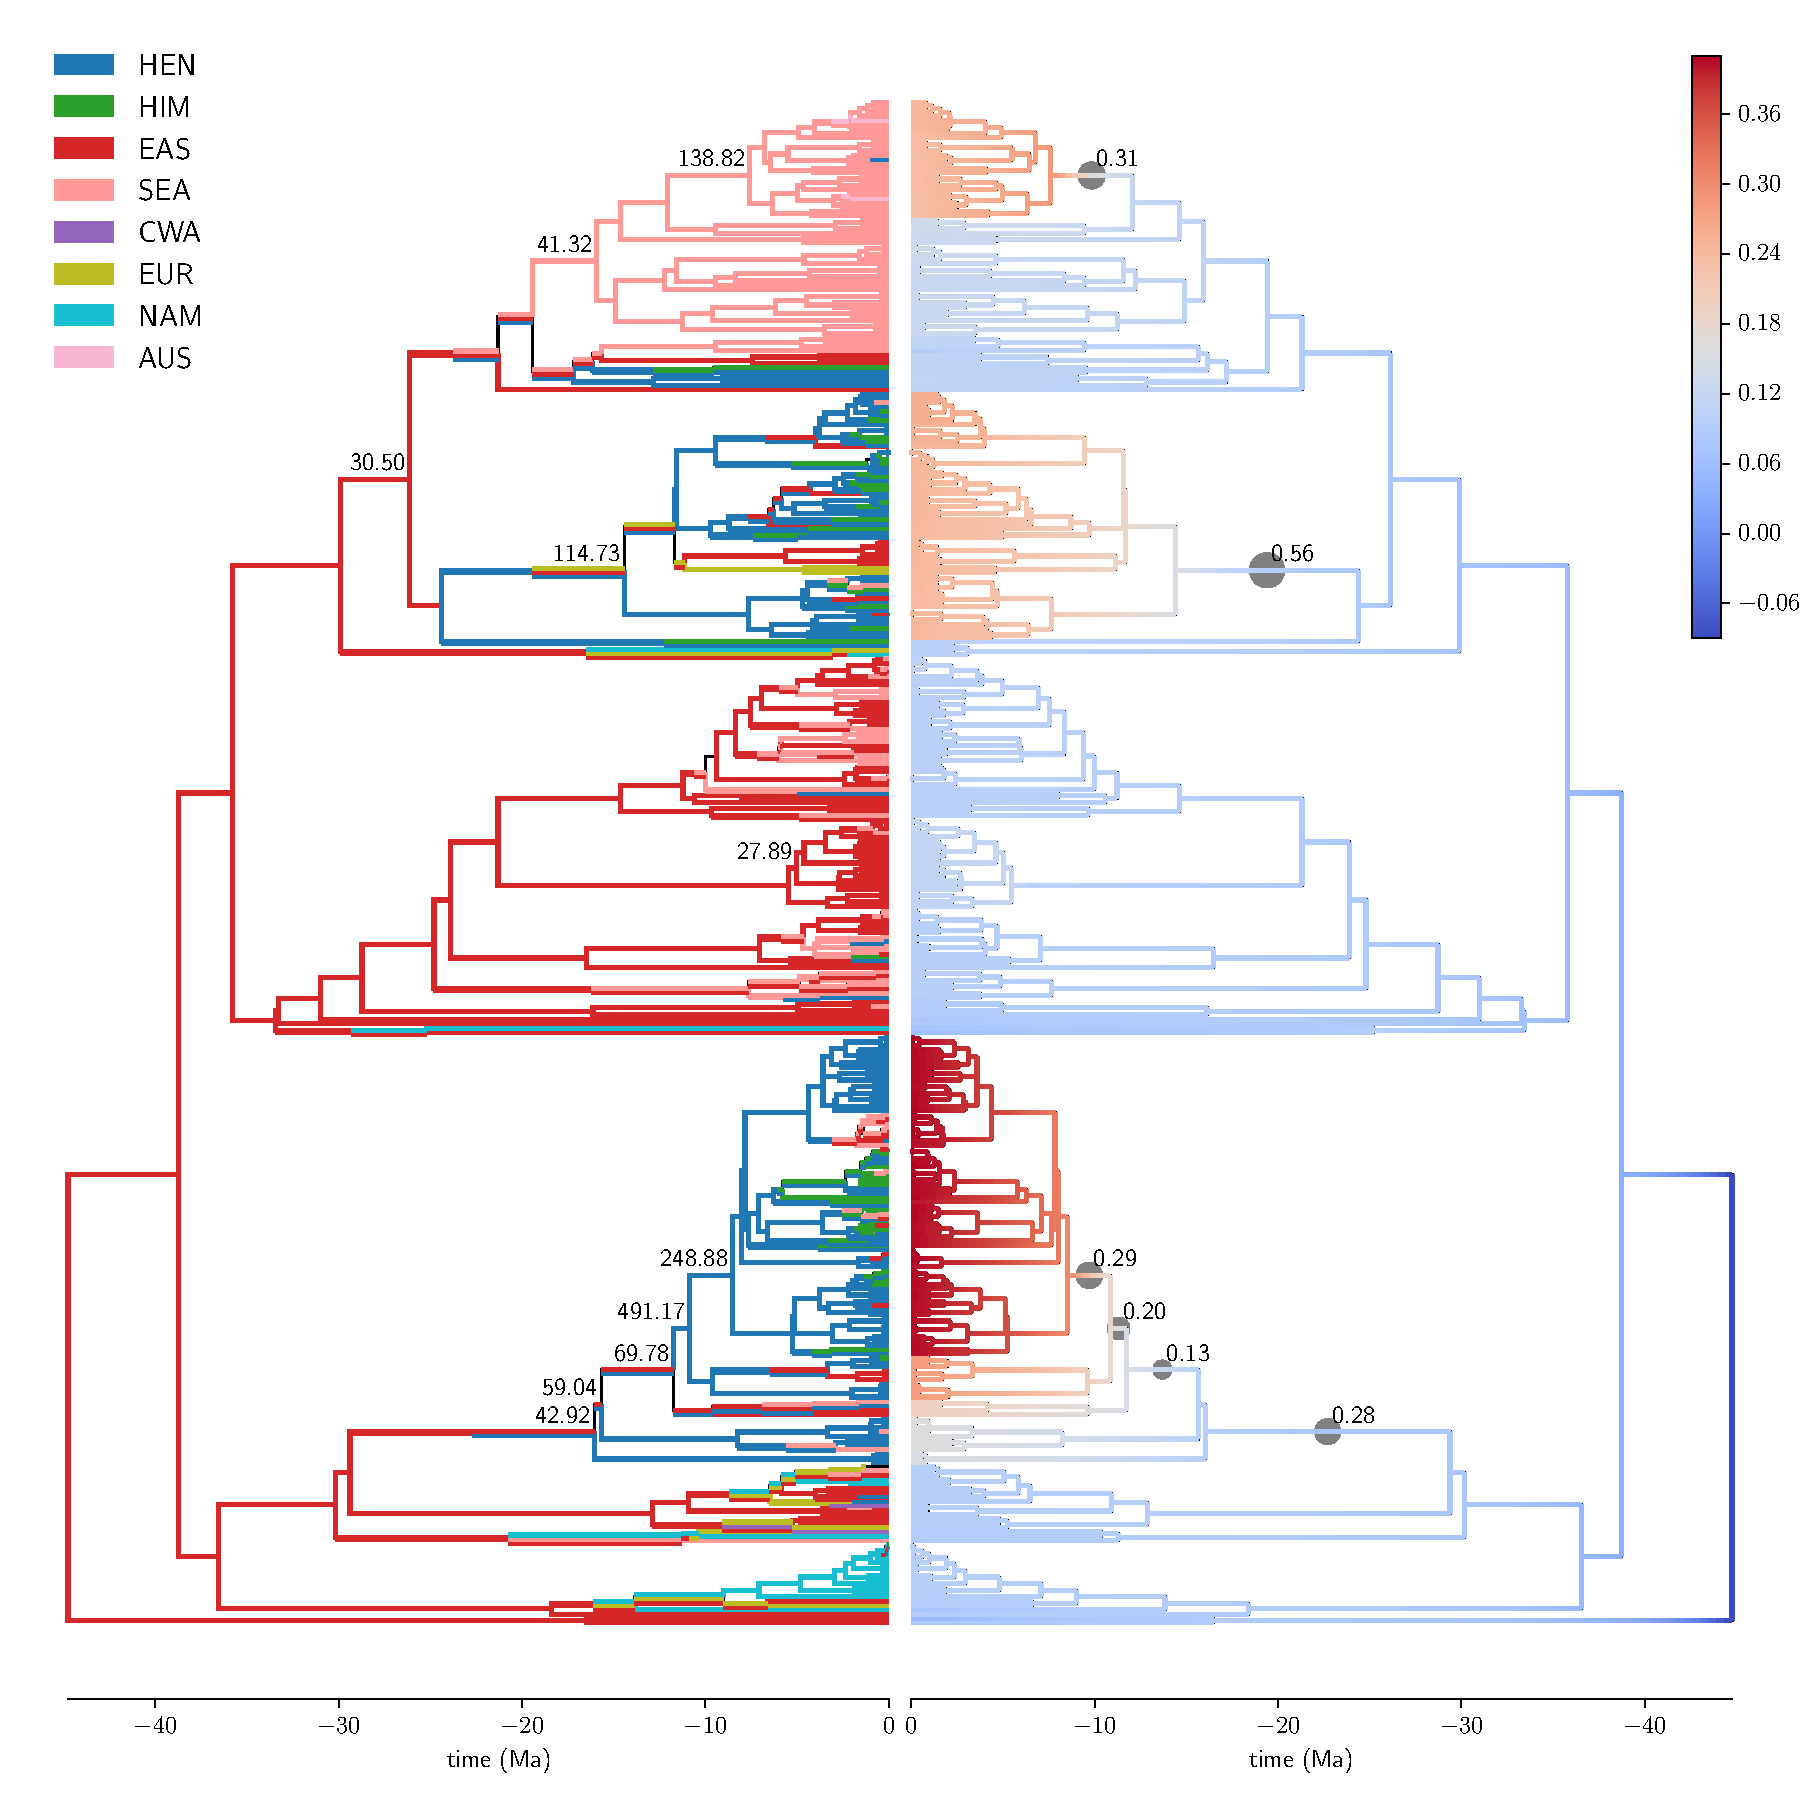
\includegraphics[width=.99\linewidth]{Rhododendron.pdf}
\caption{Reconstructions of ancestral geographic range (left) and net
  diversification rate (right) on the maximum clade credibility tree,
  with branch lengths set to posterior means, for
  \textit{Rhododendron}. Ancestral ranges are maximum-likelihood
  estimates at the start and end of each branch. Net diversification
  values are branch-segment means of the posterior distribution
  estimated by BAMM. Filled circles on the right indicate branches
  that appear in the 95\% credible set of distinct shift
  configurations, with the size and label of a circle indicating the
  cumulative probability of the branch over all configurations in the
  credible set. On the left, the marginal odds ratio for a shift in
  diversification regime along a branch is drawn for branches where
  the ratio exceeds 20. Geographic regions are coded as follows: HEN,
  Hengduan Mountains; HIM, Himalayas-QTP; EAS, temperate-boreal East
  Asia; SEA, Southeast Asia; CWA, central/western Asia; EUR, Europe;
  IND, India; AFR, Africa; NAM, North America; SAM, South America;
  AUS, Australasia. Hengduan species cluster primarily in 2 clades,
  both of which show evidence of ancestral shifts to higher
  diversification rate in the mid-to-late Miocene.}
\label{fig:rhododendron}
\end{figure}

\matmethods{

\subsection*{Clade selection and phylogeny reconstruction}

Our criteria were that each clade (1) included a substantial number of
species that occur in the Hengduan Mountains, as well as their closest
known relatives in other biogeographic regions; (2) had sufficient
molecular data available to infer a phylogeny that was broadly
representative of the clade's taxonomic diversity and geographic
range; and (3) had fossil data suitable for molecular clock
calibration or secondary calibrations inferred from fossil dated
phylogenies. We found 19 clades---17 of angiosperms and one each of
gymnosperms (Pinaceae) and ferns (Microsorioideae)---that met these
criteria. The combined taxon sample included 4,668 ingroup species, of
which 930 occur in the Hengduan Mountains region, 703 in the
Himalayas-QTP, and 1,045 in the remainder of temperate/boreal East
Asia (see \textit{Delimitation of biogeographic regions}). Of these,
about 370 species are shared between the Hengduan Mountains and
Himalayas-QTP regions. Across clades, the proportion of species
sampled ranged from 20--97\% globally and 26--94\% for the Hengduan
Mountains region (Table S1).

For each clade, we assembled molecular sequence alignments
(\textit{Dataset S1}) and fossil calibration data, and used relaxed
molecular clock models implemented in BEAST
\citep{Drummond2012,Bouckaert2014} to generate a Bayesian posterior
sample of time-calibrated phylogenies and the associated
maximum-clade-credibility tree (MCC tree).  More detailed information
is provided in \textit{SI Text}.

\subsection*{Inference of range evolution and lineage diversification}

\subsubsection*{Delimitation of biogeographic regions}

We defined 11 biogeographic regions (Fig.~S1) to accommodate the
global distributions of the selected clades, the granularity of
available species range data, and our primary focus on distinguishing
the Hengduan Mountains region from adjacent, geologically older parts
of the QTP, especially the Himalayas. To that end we defined the
Hengduan Mountains region following Boufford \citep{Boufford2014},
bounded to the west by the Yarlung Tsangpo River in eastern Xizang
(Tibet), to the northwest by the high plateau in Qinghai, to the north
by the Tao River in southern Gansu, to the east by the Sichuan Basin,
and to the south by subtropical forests and the Yunnan–Guizhou Plateau
(Fig.~\ref{fig:map}).

We defined the complementary ``Himalayas-QTP'' region as including the
plateau itself, the Himalayas to the south, the Kunlun Mountains to
the north, and the Qilian Mountains to the northeast. Our decision to
treat the Himalayas and QTP into a single unit for biogeographic
analysis, when it is clear they have distinct geological histories, is
not ideal but reflects the fact that available data on species ranges
often lacked sufficient detail to differentiate between the Himalayas
and the QTP.

The other regions we defined are: temperate/boreal East Asia (the
eastern boreal part of Russia and temperate regions of East Asia,
including Japan and Taiwan); central/western Asia (including the
Xinjiang Uyghur Autonomous Region to the north of the Kunlun Range);
southeast Asia (including tropical regions of China, Malesia, and
Papuasia); Australasia (Australia, New Zealand, and the southwestern
Pacific); India (south of the Himalyas, including Sri Lanka); Africa;
Europe; North America; and South America (south of the Panama
Canal). We scored the geographic range of each sampled species as its
presence or absence in these regions based on floras, online
databases, and published data sets (see \textit{SI Text} and
\textit{Dataset S2}).

\subsubsection*{Ancestral range reconstruction}

We estimated ancestral geographic ranges for all ingroups using a
dispersal-extinction-cladogenesis (DEC) model in Lagrange
\citep{Ree2005,Ree2008} in which dispersal was allowed based on
spatial adjacency (Fig.~S1), and the maximum range size was set to
3. We explicitly avoided placing any temporal constraints on
dispersal, so that biogeographic inferences were independent of prior
beliefs about the ages of the Hengduan Mountains or Himalayas-QTP
regions. For each ingroup, we inferred a distribution of biogeographic
histories to account for phylogenetic uncertainty. A single history
was generated in three steps. First, a chronogram was randomly sampled
from the clade's Bayesian posterior distribution. Second, the
maximum-likelihood set of ancestral ranges (geographic speciation
scenarios) at internal nodes was estimated using Lagrange. Third,
parsimonious sequences of dispersal and local extinction events were
randomly interpolated along branches having different ancestral and
descendant ranges. This procedure yielded a complete chronology of
biogeographic events, i.e., where and when ancestral lineages moved
and underwent speciation and local extinction. To account for
phylogenetic uncertainty, one history was generated for each of 500
chronograms sampled from the posterior for each clade.

\subsubsection*{Regional assembly processes through time}

We focused our analysis on the dynamics of the Hengduan Mountains
region in comparison to the Himalayas-QTP and temperate East Asia. Our
objective was to estimate, for each region, rates of \textit{in situ}
diversification and colonization and their cumulative contributions to
biotic assembly through time, while accounting for phylogenetic
uncertainy. Taking the biogeographic histories of clades from the
ancestral-range analysis, we generated 500 pseudoreplicated joint
histories---sets of one history drawn randomly from each clade's pool
without replacement. From each joint history, we extracted the
chronology of \textit{in situ} speciation, colonization, and local
extinction events affecting the Hengduan Mountains, Himalayas-QTP, and
temperate/boreal East Asia, and binned them into 1 Myr periods. This
allowed region-specific estimates of assembly processes through
time. We calculated rolling estimates of per capita \textit{in situ}
speciation rates as $\lambda(t) = s(t)/n(t-1)$, where $s(t)$ is the
number of \textit{in situ} speciation events inferred in a region in a
1-Myr period $t$ and $n(t-1)$ is the number of inferred lineages in
the region in the previous period (the cumulative sum of \textit{in
  situ} speciation and colonization minus local extinction). We also
calculated rolling per capita rates of colonization between regions as
$d_{ij}(t) = c_{ij}(t)/n_i(t-1)$, where $c_{ij}(t)$ is the number of
inferred colonization events of area $j$ from area $i$. For all
estimates, confidence intervals (5--95\% quantiles) were calculated
from the pseudoreplicated joint histories. Our results thus do not
condition on any particular tree topologies or branch lengths, and
reflect the levels of clade support, and confidence in divergence
times, provided by the sequence data.

\subsubsection*{Geography-independent rates of diversification}

To complement the regional-process analysis and to better understand
heterogeneity in rates of lineage diversification independently of
geography, we generated Bayesian inferences of diversification rate
for each clade's maximum-clade-credibility tree, with posterior mean
branch lengths, using BAMM version 2.5 and the BAMMtools R package
\citep{Rabosky2014}. BAMM uses Markov chain Monte Carlo procedures to
jointly estimate the number, parameters, and locations of distinct
macroevolutionary regimes (rates of lineage birth and death, possibly
time-dependent) on a phylogenetic tree. It can account statistically
for incomplete taxon sampling, so we assigned sampling fractions at
the finest level of taxonomic resolution possible (see \textit{SI
  text}). Priors for speciation and extinction were set empirically
using the \textrm{setBAMMpriors} function. For all clades smaller than
500 species, we set the geometric prior on the expected number of
regime shifts to 1, as recommended in the BAMM documentation; for
larger clades we also tested a prior of 10 expected shifts. We ran
each BAMM MCMC analysis for 10 million generations with a sampling
frequency of 1/1000 and assessed convergence by visually inspecting
plots of the likelihood trace and calculating the effective sample
size after discarding the first 10\% of the run as burn-in. For each
clade, we calculated Bayes factors for the distinct numbers of regime
shifts sampled, marginal odds ratios (relative evidence in favor of a
shift) for individual branches, and the 95\% credible set of distinct
shift configurations.
}
\showmatmethods

\acknow{Y.X.\ was supported by the Boyd Postdoctoral Fellowship at the
  Field Museum and by a Swiss Advanced Postdoc.Mobility Fellowship
  (P300P3\_158528) and Pioneer Hundred Talents Program of the Chinese
  Academy of Sciences. R.R.\ was supported by NSF grant
  DEB-1119098. The authors thank D.~Boufford and three anonymous
  reviewers for valuable comments on previous drafts.}

\showacknow % Display the acknowledgments section


% \pnasbreak splits and balances the columns before the references.
% If you see unexpected formatting errors, try commenting out this line
% as it can run into problems with floats and footnotes on the final page.
%\pnasbreak

\bibliography{references}
%\bibliographystyle{ecol_let}
%\bibliographystyle{pnas2011}

\end{document}

%%% Local Variables:
%%% mode: latex
%%% TeX-master: t
%%% End:
